\documentclass{beamer}

\usepackage{amsfonts}
\usepackage{amsmath}
\usepackage{longtable}
\usepackage{csquotes}
\usepackage{standalone}

\usepackage{graphicx}
\graphicspath{{../pictures/}}

\usepackage{tikz}
\usetikzlibrary{shapes, calc, arrows, decorations.markings,
  decorations.pathmorphing, decorations, patterns, chains, snakes,
  backgrounds, positioning, fit, petri}
\newcommand{\inputpicture}[1]{\input{../drawings/#1}}

\usepackage{listings}
\lstset{language=C, basicstyle=\ttfamily, breaklines=true, keepspaces=true,
  keywordstyle=\color{blue}}

\usepackage{bytefield}

\usefonttheme{professionalfonts}
\usefonttheme{serif}
\usepackage{fontspec}
\setromanfont{CMU Serif}
\setsansfont{CMU Sans Serif}
\setmonofont{CMU Typewriter Text}

\usepackage{hyperref}
\hypersetup{colorlinks=true, linkcolor=black, filecolor=black, citecolor=black,
  urlcolor=blue , pdfauthor=Evgenii Iuliugin <yulyugin@gmail.com>,
  pdftitle=Fundamentals of Full-Platform Simulation}

\usepackage{underscore}
\usepackage{amsthm}

\subtitle{Fundamentals of Full-Platform Simulation}
\subject{Lecture}
\date{\today}

\author[Evgenii Iuliugin]{
  Evgenii Iuliugin, \small{\href{mailto:yulyugin@gmail.com}{yulyugin@gmail.com}}}
\typeout{Copyright 2021 Evgenii Iuliugin}

\usetheme{Madrid}
\setbeamertemplate{navigation symbols}{}

\makeatletter
\setbeamertemplate{footline}{%
  \leavevmode%
  \hbox{%
    \begin{beamercolorbox}[wd=.15\paperwidth,ht=2.25ex,dp=1ex,center]{author in head/foot}%
      \usebeamerfont{author in head/foot}\insertshortauthor\expandafter\ifblank\expandafter{\beamer@shortinstitute}{}{~~(\insertshortinstitute)}
    \end{beamercolorbox}%
    \begin{beamercolorbox}[wd=.77\paperwidth,ht=2.25ex,dp=1ex,center]{title in head/foot}%
      \usebeamerfont{title in head/foot}\insertshorttitle
    \end{beamercolorbox}%
  }%
  \begin{beamercolorbox}[wd=.08\paperwidth,ht=2.25ex,dp=1ex,right]{date in head/foot}%
    \usebeamerfont{date in head/foot}%
    \usebeamertemplate{page number in head/foot}%
    \hspace*{2ex}
  \end{beamercolorbox}
  \vskip0pt%
}
\makeatother

\newcommand{\startslides}{
  {\setbeamertemplate{footline}{}
  \begin{frame}
      \maketitle
  \end{frame}
  }

  \addtocounter{framenumber}{-1}

  \begin{frame}{\inserttitle}
      \tableofcontents
  \end{frame}
}

\newcommand{\finalslide}{{
  \setbeamertemplate{footline}{}

  \begin{frame}

  {\huge{Thank you!}\par}

  \vfill
  Slides and material are available at
  \url{https://github.com/yulyugin/sim-lectures}
  \vfill

  \tiny{\textit{Note}: All trademarks are the property of their respective
    owners. The presented point of view reflects the personal opinion of
    the author.

    %All the materials are licensed under the Creative Commons
    %Attribution-NonCommercial-ShareAlike 4.0 Worldwide. To view a copy of this
    %license, visit \url{http://creativecommons.org/licenses/by-nc-sa/4.0/}.
  }
  \end{frame}
}\addtocounter{framenumber}{-1}}


\title{Параллельная симуляция. Многопроцессорные гостевые системы}

\begin{document}

\startslides

\begin{frame}{On the Previous Lecture:}
  Programming languages for model developemnt:
  \begin{itemize}
    \item Requirements and abstructions.
    \item Libabries: SystemC.
    \item Domain specific languages: DML, SimGen, LISA.
    \item Languages for hardware development: VHDL, Verilog.
  \end{itemize}
\end{frame}

\begin{frame}{Questions}
\end{frame}

\begin{frame}{Earlier in the Course}
  \begin{itemize}
   \item Simulation of multi-processor systems\dots\pause
   \item \dots using just one host processor core.
   \vfill
   \item $N$ target cores are simulated sequentially on $K$ host cores.
   \item Slowdown may be $> \frac{1}{N}$.
   \item At the same time $K-1$ host cores are unused.
  \end{itemize}
\end{frame}

\begin{frame}{Simulated System}
  \centering
  \inputpicture{parsim-overview}
\end{frame}

% \begin{frame}{Препятствия}
% \begin{enumerate}
% \item    Возможность гонок данных (data race)
% \item    Возможность взаимоблокировок
% \item    Неэффективная работа параллельного приложения
% \item    Недетерминистичность
% \end{enumerate}
% \end{frame}

\section{Processors Simulation}

\subsection{Atomic Instructions}

\begin{frame}{Atomic Instructions}
  \centering
  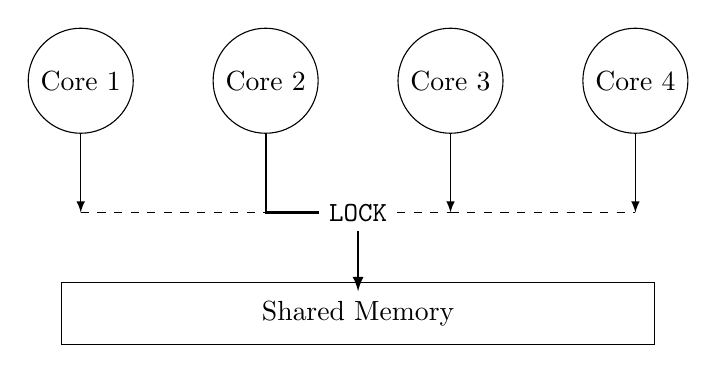
\begin{tikzpicture}[>=latex]
    \node[draw, circle] (core1) {Core 1};
    \node[draw, circle, right = of core1] (core2) {Core 2};
    \node[draw, circle, right = of core2] (core3) {Core 3};
    \node[draw, circle, right = of core3] (core4) {Core 4};

    \path (core2.south) -- (core3.south) node[midway, yshift = -1cm] (lock) {\texttt{LOCK}};
    \draw[thick] (core2) |- (lock);

    \node[below = 1cm of lock.center] (shmem) {Shared Memory};
    \node[inner ysep=0pt, below = 2cm of core1.south] (c1) {};
    \node[inner ysep=0pt, below = 2cm of core4.south] (c2) {};
    \node[draw, fit = (c1) (shmem) (c2)] {};

    \draw[thick,->] (lock) -- (shmem);

    \path (core1.south) |- (lock) coordinate[midway] (block1);
    \path (core3.south) |- (lock) coordinate[midway] (block3);
    \path (core4.south) |- (lock) coordinate[midway] (block4);

    \draw[->] (core1.south) -- (block1);
    \draw[->] (core3.south) -- (block3);
    \draw[->] (core4.south) -- (block4);

    \draw[dashed] (block1) -- (lock);
    \draw[dashed] (lock)   -- (block3);
    \draw[dashed] (block3) -- (block4);
  \end{tikzpicture}

  \begin{itemize}
    \item {Read--Modify--Write} memory.
    \item Atomic instructions --- <<all or nothing>>.
    \item Atomic instructions are <<expensive>>.\pause
    \item Question: Do single core systems need atomic operations?
  \end{itemize}
\end{frame}

\begin{frame}{Simulation of atomic instructions}
  \begin{enumerate}
    \item Using host atomic instructions.
    \begin{itemize}
      \item Different ISAs for atomic instructions (Intel IA-32 --- 10+ atomic
        instructions, ARM --- two).
      \item Usefull when target and host architectures match. \pause
    \end{itemize}
    \item Using critical sections.
    \begin{itemize}
      \item Atomic instruction acquires a lock before memory access \pause
        \dots{} does not work. See~\cite{coremu}.
      \item Every memory access acquires a lock --- works but slow. \pause
      \item Coherency protocols for memory regions. Like MESI for caches. \pause
    \end{itemize}
    \item Using transactions.
    \begin{itemize}
      \item Detect races instead of avoiding them.
      \item Repeat atmoic operation in case of failure.
      \item Implemented using host atomic compare-and-swap.
    \end{itemize}
  \end{enumerate}
\end{frame}

\subsection{Memory Models}

\begin{frame}{Memory Consistency Models}
  \begin{itemize}
    \item There are several buffers (caches, queues) between CPU and RAM.
    \item CPUs in a shared memory system may <<see>> different values of the
      same memory location.
    \item Memory consistency model --- set of rules defining order and
      visibility of memory updates.
    \pause
    \vfill
    \item Memory barriers --- instructions to establish partial ordering for
      memory operations.
    \item Examples Intel\reg~IA-32: \texttt{sfence}, \texttt{lfence},
      \texttt{mfence}.
    \item NOTE: atomic instructions are not necesserely memory barriers!
  \end{itemize}
\end{frame}

\begin{frame}{Memory Ordering for Different Architectures}
  \centering
  % TODO: Convert the table to LaTex
  \includegraphics[height=0.8\textheight]{barrier-arch.png}

  \tiny{Summary of memory ordering~\cite{whymb}}
\end{frame}

\section*{Conclusion}

\begin{frame}{Parallel Simulators}
  \begin{itemize}
    \item Simics
    \item Graphite
    \item SimOS
    \item Coremu
    \item Pqemu
    \item BigSim
    \item DynamoRIO
  \end{itemize}
\end{frame}

\begin{frame}{Conclusion}
\end{frame}

\begin{frame}[allowframebreaks]{Bibliography}
  \begin{thebibliography}{99}
    \bibitem{coremu} \textit{Zhaoguo Wang et al.} COREMU: a Scalable and Portable Parallel Full-System Emulator \url{http://ppi.fudan.edu.cn/_media/publications\%3Bcoremu-ppopp11.pdf},
    \bibitem{consistency-report} \textit{Kourosh Gharachorloo} Memory Consistency Models for Shared-Memory Multiprocessors. \url{http://infolab.stanford.edu/pub/cstr/reports/csl/tr/95/685/CSL-TR-95-685.pdf}
    \bibitem{whymb} \textit{Paul E. McKenney} Memory Barriers: a Hardware View for Software Hackers \url{http://citeseerx.ist.psu.edu/viewdoc/summary?doi=10.1.1.152.5245}
    \bibitem{pqemu} \textit{Jiun-Hung Ding et al.} PQEMU: A Parallel System Emulator Based on QEMU \url{http://dx.doi.org/10.1109/ICPADS.2011.102}
  \end{thebibliography}
\end{frame}

\finalslide

\end{document}
